% Here comes two of you,
% which one will you chose?
% One is black, one is blue.
% I'm beginning to see the light - Velvet Goldmine

% Not all good things come to an end now it is only a chosen few

%And do you think it's so easy to find
%Somebody who is just your kind
%Oh, it might take you a little time
% Pulp - happy endings



% All the people are dancing
% and they're having such fun
% I wish it could happen to me
% after hours - velvet u

\section{Working with a real Web radio}

This chapter is divided in two parts.
The first two sections describe the experience of ten actual users with Poolcasting Web radio: which channels they created, which songs they shared, which impressions they perceived.
The rest of the chapter reports of experiments to evaluate how poolcasting can deliver radio channels that address the goals of customisation and fairness.
A particular attention is dedicated to measure how the size and the musical homogeneity of the audience can affect the group satisfaction.

\subsection{The active audience} % (fold)
\label{sub:the_audience2}

An implementation of Poolcasting Web radio has been running for one year on a Web server located in the internal network of the Institut d'Investigaci\'{o} en Inte\lgem ig\`{e}ncia Artificial (IIIA-CSIC).
The radio has been showcased in different research institutes, % (IIIA-CSIC, Queen Mary University, University College of London), to
music-related companies % (MusicStrands, Last.fm) 
and international conferences \cite{Baccigalupo07c,Baccigalupo07e,Baccigalupo07f};
% The radio requires users to authenticate; 
at each presentation the audience was asked to join and evaluate the system. A total of 29 persons accepted, ten of which have connected to the radio more than once. 
These `active' users are male and 30 years old in average; five are Italian, four are Spanish and one is English.
% subsection the_audience2 (end)

\subsection{The music pool} % (fold)
\label{sub:the_music_pool}

Eight of the ten participants agreed to share on the radio the songs contained in their personal music libraries.
The total number of shared songs was 60,202. 
Matching these titles against OpenStrands and Last.fm Web services and discarding duplicates reduced the size of the music pool to 24,763 songs.

Five of the eight shared libraries were online 24 hours a day since they were stored on computers that were never switched off; the remaining three libraries were instead only available when the computers where they reside were connected to the Web.

%According to the data stored in the respective iTunes libraries, 
The most common genres for the songs in the music pool were: Rock (3,499 songs), Soundtrack (2,670), Pop (1,609), Alternative \& Punk (1,156), Electronic (614), Alternative Rock (560) and Indie (504). 
Most songs were published in 2005 (1,642 songs), while the average year of publication was 1999.
%
%According to the data retrieved from 
Matching the music pool against Last.fm Web service revealed the following tags as the most common: rock \& pop (9,138 songs), alternative (1,402), international (1,178), hard rock (529), r\&b (520).

% subsection the_music_pool (end)

\subsection{Listening habits} % (fold)
\label{sub:listening_habits}

The listening habits data stored in the shared libraries revealed that most participants had never played or rated the songs contained in their libraries.

Only 4,564 of the 24,263 songs (18.4\%) had ever been played by their owners in iTunes, while only 358 songs (1.4\%) had been rated. % with a certain number of `stars'.
The average play count for the 4,828 songs that had ever been played or rated was 1.8 times while the average rating was 3.3 stars.

These data interestingly point out how people may hold large music libraries in their hard disks and still play and rate only a small amount of songs, leaving most of their music collection untouched.

%select count(*) from archives where itunes_count is not null and library_id in (1,2,3,5,7,13,10,12,15) and song_id is not null;

% subsection listening_habits (end)

\subsection{Observations} % (fold)
\label{sub:observations12}

Although the radio was presented to about 100 persons, only ten became active participants.
Informal interviews to those who did not join the radio revealed two main reasons. 
Some people were unfamiliar with online radios and were not interested in trying a new one. Others appreciated the idea of a social Web radio but did not have a music library managed with Apple iTunes, so could not actively participate. % to poolcasting.

The ten active users showed a noticeable interest for Poolcasting Web radio, to which they connected day after day.
The number of shared songs was quite large compared to the number of listeners (in average 2,476 tracks per user), which enabled people to frequently discover unknown music.

A negative characteristic related to the active users was the low rate of played and rated songs in their personal libraries, which allowed poolcasting to build only partial models of their music profiles, restricted to a few songs and artists. 
The feedback provided through the `Good' and `Bad' buttons on the Web interface resulted very important to refine these music profiles over time.


% subsection observations12 (end)


\section{Variety and smoothness} % (fold)
\label{sub:active_channels}

Fifteen distinct channels were created by the ten active users of the radio. 
Most channels were defined as single-genre (e.g., `Rock' channel); others using periods (e.g. `Music from the Eighties'); others combining genres and tags (e.g., a `Soundtracks' channel playing tracks tagged as `Soundtrack', `Sound track', `Banda Sonora' or `BSO'\footnote{`BSO' stands for `Banda Sonora Original', `Original Soundtrack' in Spanish.}).
Although participants could alter the definition of a channel after its creation, this function was barely used.

\subsection{Variety} % (fold)
\label{sub:variety2}

The variety of the music played on each channel (\ref{p:variety}) was achieved by setting the repetition parameters to $\eta = 50$ and $\zeta = 5$ (see Sect.~\ref{sec:the_case_based_reasoning_selection_process}): every song could be repeated on the same channel only after 50 other songs, while songs by the same artist had to be separated by at least 5 songs.
These values were meant to avoid short-term repetition of the same music.

A problem reported by some listeners was that channels would sometimes repeat the same \emph{sequence} of songs in consecutive days.
For instance, whenever `Romeo Had Juliette' (Lou Reed) played in the `Rock' channel, it was always followed by `The Wait' (The Pretenders).

The reason for this behaviour is that `The Wait' is the top associated song with `Romeo Had Juliette' in the music pool according to the knowledge in the data set of playlists.
This means that, in the retrieve process, `The Wait' always ranks as the best candidate to follow `Romeo Had Juliette' and, in the reuse process, is the song selected to play next, unless the audience explicitly states a negative feedback.

To avoid this unpleasant behaviour, the requirement for variety was strengthened, forbidding that any \emph{pair of consecutive songs} could be repeated two times in a row in the same channel.
The song `Romeo Had Juliette', for instance, would be followed by `The Wait' (the top associated song) on its first appearance in the `Rock' channel, 
while it would be followed by `The Same Situation' (Joni Mitchell)\,---\,the second top associated track\,---\,on its second occurrence, and so on.
This enabled the radio to achieve both short-term and long-term variety.

\subsection{Smoothness} % (fold)
\label{sub:smoothness2}

Poolcasting Web radio reuses the musical associations extracted from the analysis of playlists (see Chap.~\ref{cha:smoothness}) to address the requirement of smoothness (\ref{p:smoothness}). 

An example of smooth musical sequence delivered on the `Rock' channel was: `Pretty Noose' (Soundgarden), `Bullet with Butterfly Wings' (Smashing Pumpkins), `Kool Thing' (Sonic Youth), `MFC' (Pearl Jam), `Medication' (Queens of the Stone Age).
This sequence shows a certain continuity since all these songs revolve around the U.S. Indie Rock sound of the Nineties and go well together both for acoustic and cultural reasons.

Imposing smooth transitions from song to song comes at a price: the influence of the listeners is narrowed to decide only among a few candidates. As a result, a channel can take a long time to adapt content to the audience.

An example was reported by an active user of the `Rock' channel who had to wait for the duration of four songs (about fifteen minutes) before listening to an Electronic Rock track, akin to his musical profile.
The reason was that, because of the smoothness requirement, poolcasting could not `jump' directly from one style to another but had to pass through a series of intermediate tracks before reaching an Electronic Rock track.

To avoid this behaviour, the smoothness requirement in Poolcasting Web radio was relaxed to include randomly chosen tracks in the retrieved set as well as songs that were musically related to the previous one.
Specifically, the retrieve process was modified to retrieve the top 10 candidates from the list of associated tracks and the last 5 candidates at random from the channel pool.
If the listeners ranked any of these songs better than the rest, that song would be played next, even without being the most associated with the last one.
%
The Electronic Rock lover of the previous example, for instance, could in this way browse the retrieved set and pick the random candidate which was most akin to his musical taste, rapidly bending the music towards a more Electronic style.

With this approach, faster transitions could occur from a sub-genre to another when persons with different musical taste were present in a channel.

% subsection active_channels (end)

\subsection{Observations} % (fold)
\label{sub:subjective_evaluation}

Other characteristics that the audience particularly appreciated or objected were revealed in a series of interviews to the radio listeners.

% PAU
One participant found among the greatest qualities of Poolcasting Web radio ``the idea of taking music out of personal libraries to new listeners''. This was seen as a great way to get to know new composers and songs. Another quality was the ``direct participation of the listener, which makes it a social radio''.
The main drawbacks observed were that ``a channel can rapidly become overcrowded, negatively affecting individual satisfaction'' and also the fact that musical preferences assessed from iTunes libraries can be wrong when the users are not ``careful with their content, which can badly affect the quality of the transmission''.

% NEAL
A different participant replied that the best aspects of the radio were ``the interface, the streaming audio quality and the social aspect of the radio, even though I did not have the chance to fully delve into this''. The worst aspect found was ``having to wait for songs I did not like to finish''. The participant also commented that ``this kind of radio would work best in a shared office, where people are not just interacting \emph{online} as they listen to the music''.
%+ very few channels..

% MANU
A third participant rated positively the ``comfortable interface'', while was worried about the long time that had to pass before the radio could learn individual musical preferences. 
In his opinion, Poolcasting Web radio can make listeners ``quite satisfied'' but not ``totally satisfied'', something that is positively ``compensated by getting to discover new music that you are probably going to like''.

%-Interfaz muy cómoda y agradable de ver.
%-La sensación que me queda es que hay que estar mucho tiempo escuchando la radio para que pueda aprender tus preferencias.
%-Creo que la radio sólo puede llegar a tenerte "lo suficientemente satisfecho", pero no "totalmente satisfecho". De todas maneras, esto ya es suficiente, cuando la recompensa es conocer canciones nuevas de grupos que seguro que te van a gustar.
%Detalles menores:
%-Cada vez que la canción cambia es necesario volver a pulsar el botón de play para escuchar la música.
%-Sólo por azar se da uno cuenta que hacer dos veces click en bad no es lo mismo que bad. ¿Por qué no poner directamente "very bad" y "very good"?
% Dudas:
%-¿Poolcasting utiliza la librería del usuario para aprender? ¿O era algo que has hecho después?


% CLAUDIO
A fourth participant appreciated the fact of being able to ``rediscover songs from the bottom of my music library, that I did not remember having''.
\citet{Voida06} already investigated the satisfaction given by this ``rediscovery'' experience which is correlated to the increasingly large music libraries that characterise several iTunes users.

The main lesson learnt is that the listeners of Poolcasting Web radio implicitly accept a social compromise. When they join a channel, they are aware they will not possibly like every song played, yet they will have the chance to easily discover new music preferred by other listeners, with whom they can interact and discuss.
This social component would not exist if they were to play music directly from their personal digital players or from other Internet radios.

% subsection observations94 (end)

% 
% 
% 
% \paragraph{Example of customisation.} % (fold)
% \label{par:example_of_customisation_}
% Some experiments. The first one is the following: I set up the same channel with the same library, but in one case I have no user modelling (all neutral), in the other I have it, and I observe how things change (using a deterministic choice, always the first candidate).
% 
% without: Pretty Noose (Soundgarden) -> Bullet with Butterfly Wings (Smashing Pumpkins) -> Kool Thing (Sonic Youth) -> (Drawing) Rings.. (Super Furry Animals) -> Everybody's Got Something.. (The Beatles) -> MFC (Pearl Jam) -> Medication (Queens of the Stone Age)
% 
% with personalisation (and I like electronic apart from Rock): Pretty Noose (Soundgarden) -> Elderly Woman.. (Pearl Jam) -> Kool Thing (Sonic Youth) -> Seventeen (Ladytron) -> Tribulations (LCD Soundsystem) -> 23 (Blonde Redhead) -> Objects of my affection (Peter Bjorn \& John).
% % paragraph example_of_customisation_ (end)
% 
% % subsection subjective_evaluation (end)
% 
% [TO DO: Experiments with the SYSTEM, such as each channel requires this amount of memory, on a G4 only 4 channels can run simultaneously, etc.]
% 
% % section experiments_with_the_radio (end)


\section{Group customisation and fairness} % (fold)
\label{sec:evaluation_of_this_technique}

The previous section reported on experiences of real users of Poolcasting Web radio and on the way in which radio channels achieve a level of variety (\ref{p:variety}) and smoothness (\ref{p:smoothness}) that is appropriate for the audience.
%
The rest of the chapter evaluates whether the poolcasting technique can achieve the goals of customisation (\ref{p:customisation}) and fairness (\ref{p:fairness}) on groups of different sizes and musical homogeneity.

To obtain objective results, independent of the particular music profiles of the ten active users, the evaluation is run in a simulated environment with a set of artificially created profiles.

% Each profile is generated with random music preferences, that is, each user is designed to like some songs and dislike other ones at random. 
% More precisely, the preference degrees $i(U,X)$ of each artificial user $U$ for each song $X$ have been generated as a uniformly random distribution of numbers in $[-1,1]$, as illustrated in Fig.~\ref{fig:unif_dist}
% %
% \begin{figure}[bthp]
% \centering \setlength{\abovecaptionskip}{3pt}
% \epsfig{file=img/unif_dist, width=\textwidth}
% \caption{Uniform distribution of preference degrees [CHANGE].}
% \label{fig:unif_dist}
% \end{figure}
% % x <- sort(runif(1000))*2-1; plot(x,dnorm(x=x,sd=0.5),type="l",ylim=c(0,1))
 
%The evaluation is run by creating a radio channel with a certain number of `fake' listeners, running the CBR process that chooses which songs to play according to their preferences and finally analysing whether poolcasting has achieved its purpose of adapting the music to the audience (\ref{p:customisation}) and having all the user satisfied over time (\ref{p:fairness}).

\subsection{Random music profiles} % (fold)
\label{sub:initial_configuration}


The first experiment evaluates the performance of poolcasting in a radio channel with five participants.
Each person is simulated by an artificial music profile that describes which songs a participant likes and dislikes.
Precisely, five music profiles are generated \emph{randomly}, that is, assigning a random number in $[-1,1]$ to the individual preference $i(U,X)$ of each participant $U \in \mathcal{U}$ for each song $X \in \mathcal{C}$.

This is intended to emulate a sort of worst case scenario where five members of a channel do not share any particular musical affinity: one may like some Pop and Rock songs and detest Heavy Metal tracks, another may like Jazz and Rock and dislike Pop, and so on.

The five participants all join the same radio channel, defined with no filter: all the available music is allowed to play, from any genre, year or tag.
The channel is started, and the first song is played at random from the available ones.
%
All the successive songs are selected by the poolcasting CBR technique described in Sect.~\ref{sec:the_case_based_reasoning_selection_process}, with the parameters initially set to $\kappa = 15$ (size of the retrieved set), $\iota = 0.4$ (initial satisfaction), $\chi = 0.8$ (satisfaction decay) and $\mu = -0.75$ (misery threshold).

Whenever a new song is played, the values of two functions are registered for every participant $U$:
\begin{itemize}
 \item $h(U,T)$, that is, how much $U$ likes the song played; and
 \item $q(U,T)$, that is, how satisfied $U$ is for the songs played so far.
\end{itemize}

After $25$ songs, the channel is stopped and the registered values are analysed.
In order to obtain significant results, the whole process (creating a channel, playing 25 songs, collecting results) is replicated 20 times with different initial random songs and music profiles and the analysis is performed on the average values of $h(U,T)$ and $q(U,T)$ through all the iterations.

This experiment is meant to evaluate whether poolcasting can fairly satisfy a group of five listeners characterised by random music profiles.
This can be considered as a sort of worst case scenario since in the real world listeners of the same radio channel typically share some musical affinity.

\subsection{Results} % (fold)
\label{sub:initial_results}

Figure~\ref{fig:default} shows the result of this evaluation.
Each line in the graph corresponds to one of the five participants. 
The plot on the left shows the individual preferences $h(U,T)$ of each participant for each of the 25 songs played; the plot on the right indicates their satisfaction degrees $q(U,T)$ after each song.
%
\begin{figure}[bthp]
\centering \setlength{\abovecaptionskip}{3pt}
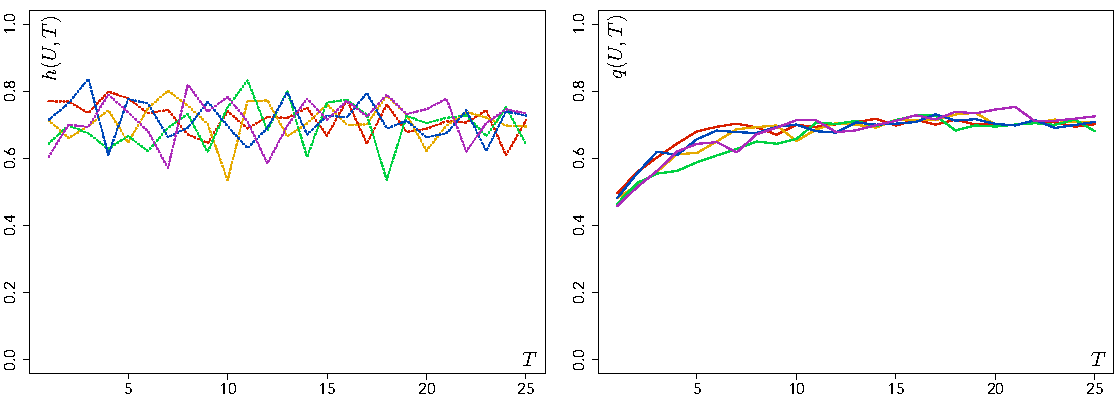
\epsfig{file=img/fig6_1, width=\textwidth}
\caption{Individual preferences and satisfaction degrees of five participants listening to the same channel for the duration of 25 songs.}
\label{fig:default}
\end{figure}

With regard to customisation, the results look positive.
The whole audience likes every song, %more or less 
with an average individual preference of
% means = apply(preferences, c(1,2), mean, na.rm=TRUE)
$\overline{h(U,T)} = 0.72$.
%
Lower spikes in Fig.~\ref{fig:default} (left) indicate songs that a participant did not particularly like; even in these occasions the preference $h(U,T)$ never falls below a value of $0.5$.
Moreover, lower spikes are immediately followed by high values, demonstrating the power of poolcasting in rewarding participants who did not like some of the recently played songs.

The impact of this balanced strategy over individual satisfactions is illustrated in Fig.~\ref{fig:default} (right).
All the lines are quite close and stable over time, indicating that poolcasting achieves fairness by keeping every participant similarly satisfied in the long run.

% The standard deviation of $h(U,T)$ for all the songs and participants is as low as $0.05$.

The difference between the most and the least satisfied listener is small: $q(U,T)$ has an average standard deviation of $0.04$ which means that a reasonable degree of fairness is achieved.
The satisfaction of the group as a whole is quite high for this kind of worst case scenario, in fact the average satisfaction degree over the 25 songs played equals $\overline{q(U,T)} = 0.68$.


\section{Discordant listeners} % (fold)
\label{sec:discordant_listeners}
 
The previous section has evaluated poolcasting on a group of listeners with random individual preferences. 
In that case, poolcasting was able to deliver a group-customised sequence of songs to satisfy the entire audience.

This section considers a different situation in which five participants are split into two purely antagonist groups: the music that three users prefer, the other two dislike, and vice versa. No song exists that the entire audience likes.

The rationale of this experiment is to prove whether poolcasting can achieve fairness with discordant listeners, determining a sequence of songs that, in the long run, can match the preferences of all the participants.
Again, this is a sort of worst case scenario: in the real world, listeners of the same radio channels typically share musical affinities for some songs.

For the sake of this experiment, five artificial profiles are created to simulate five participants split into two discordant groups.
Three users are assigned with random \emph{positive} preferences $i(U,X)$ for half of the available songs and with random \emph{negative} preferences for the remaining half; the opposite occurs for the other two users.

Figure~\ref{fig:random} (left) illustrates this distribution on a sample set of ten songs: the users labelled as 1, 2 and 3 only like the last five songs, while the users labelled as 4 and 5 only like the first five songs.
By comparison, Fig.~\ref{fig:random} (right) represents the scenario previously evaluated in Sect.~\ref{sec:evaluation_of_this_technique} where individual preferences were independently assigned among listeners.
%
\begin{figure}[bthp]
\centering \setlength{\abovecaptionskip}{3pt}
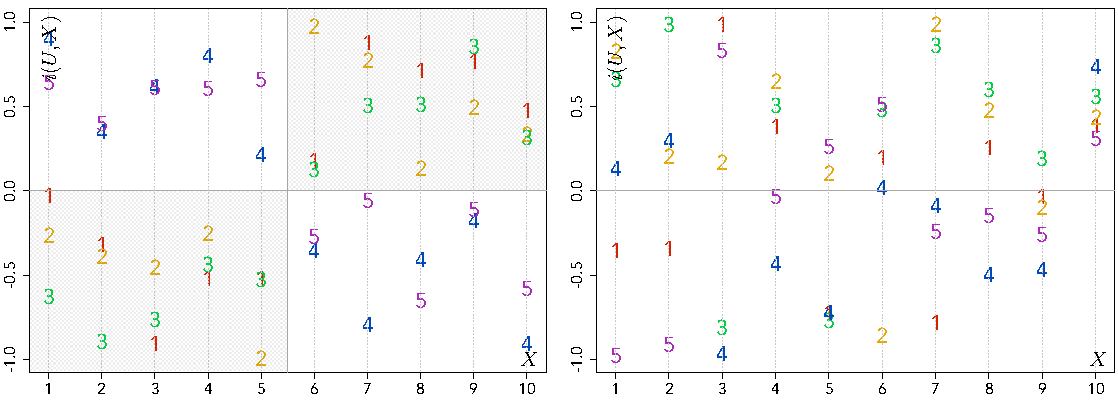
\epsfig{file=img/fig6_2, width=\textwidth}
\caption{Sample individual preferences of five participants whose profiles belong to two discordant groups (left) or are independent (right).}
\label{fig:random}
\end{figure}

The evaluation is run as in Sect.~\ref{sec:evaluation_of_this_technique}, having the channel playing $25$ songs, repeating the process $20$ times with different initial songs, and observing the values of $h(U,T)$ and $q(U,T)$ at each iteration. 
%The only difference is in the creation of the artificial user profiles.  Rather than simply having random preference degrees, in this case a majority of the audience (three listeners) has random \emph{positive} preferences for half of the music pool and random \emph{negative} preferences for the rest, while the opposite occurs for the minority (two listeners).

\subsection{Results} % (fold)
\label{sub:results73}

The results of the evaluation are shown in Fig.~\ref{fig:fair_1}: 
the plot on the left marks the individual preferences $h(U,T)$ for the songs played; the plot on the right indicates the satisfaction degrees $q(U,T)$ of the five participants.
%
\begin{figure}[bthp]
\centering \setlength{\abovecaptionskip}{3pt}
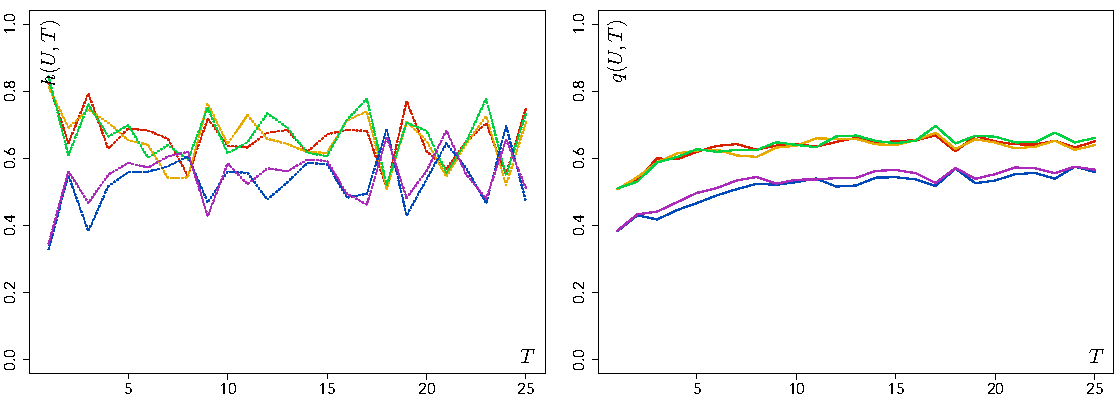
\epsfig{file=img/fig6_3, width=\textwidth}
\caption{Individual preferences and satisfaction degrees of five participants split in two groups with discordant music profiles.}
\label{fig:fair_1}
\end{figure}

%\subsection{Observations} % (fold)
%\label{sub:observations9}

The first observation is that the two groups can be clearly identified in the graphs: most played songs are preferred by three participants who, as a consequence, have a higher satisfaction degree.

Still, the difference between the two groups is not very large and whenever a song preferred by the majority is played, a song preferred by the minority is played soon after. 
The songs played at position 8, 18, 21 and 24, for instance, are preferred by the minority more than by the majority. %, as shown in Fig.~\ref{fig:fair_1} (left).
Moreover, every song played, although preferred by one of the two antagonist groups, has been selected to be reasonably acceptable by the members of the other group, albeit to a lesser degree.

The motivation for this balanced outcome is the satisfaction-weighted aggregation strategy presented in Sect.~\ref{sec:social-choice-problem} that combines individual preferences rewarding less satisfied listeners.
In this case, two participants are generally less satisfied than the other three so once in a while poolcasting delivers one of their favourite songs, to achieve fairness.

Thanks to this approach, the distance between the satisfaction degrees of the groups does not increase over time, as shown in Fig.~\ref{fig:fair_1} (right). 
This result is notably positive considering that actual radio channels do not typically have an audience split into two purely antagonist groups.

\subsection{The importance of memory} % (fold)
\label{sub:comparison_with_plurality_voting}

In the previous experiment, a certain degree of fairness was achieved thanks to the satisfaction-weighted aggregation strategy that holds memory of previous outcomes to determine which items to deliver next.

To prove that this strategy is the responsible for the positive results obtained, an equivalent experiment is run under the same conditions but using a different aggregation strategy, with no memory of past decisions.

The experiment is run with the same audience of two discordant groups but preferences are here combined with a simpler approach, selecting at each step the song that has \emph{in average} the highest preference, independently of the previous songs played. No memory of past satisfaction is kept.

The results of this experiment are shown in Fig.~\ref{fig:fair_2} which illustrates the average individual preferences (left) and satisfaction degrees (right) of the five participants for the songs played.
%
\begin{figure}[bthp]
\centering \setlength{\abovecaptionskip}{3pt}
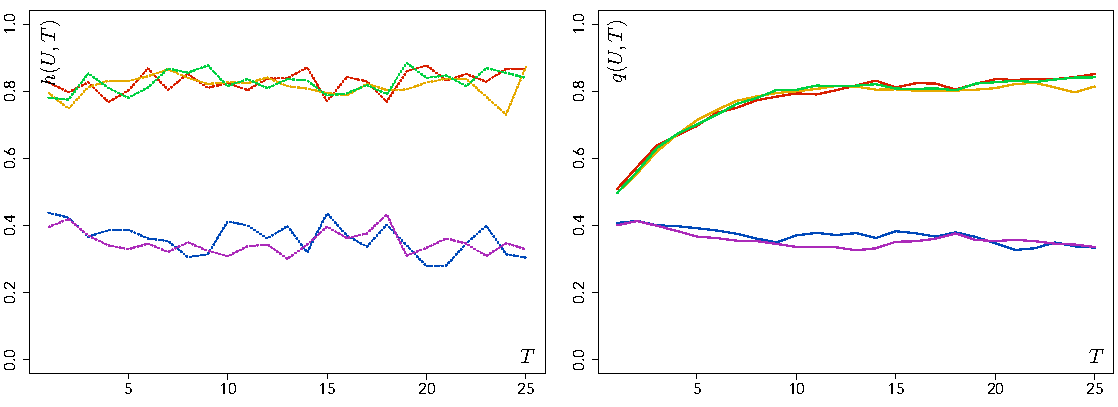
\epsfig{file=img/fig6_4, width=\textwidth}
\caption{Individual preferences and satisfaction degrees of five discordant participants when songs are selected without memory.}
\label{fig:fair_2}
\end{figure}

As can be observed in Fig.~\ref{fig:fair_2} (left), in this case the radio channel plays only songs that three participants (the majority) prefer more than the remaining two (the minority).
As a consequence, three members of the audience are more and more satisfied as time goes by, while the remaining two members are less and less satisfied, as shown in Fig.~\ref{fig:fair_2} (right).

The lesson learnt is that, without memory of past elections, fairness can only be achieved punctually, satisfying at each moment only the current majority.
The satisfaction-weighted aggregation strategy that characterises poolcasting, on the other hand, can fairly satisfy the entire audience over time, playing songs that both the majority and the minority like to a certain extent.

% subsection observations9 (end)

% subsection fairness (end)

\section{Concordant listeners} % (fold)
\label{sub:concordance}

The next experiment is meant to evaluate the performance of poolcasting in the case members of the audience share some affinity with respect to their music profiles.
While the previous sections focused on worst-case scenarios made of random or antagonist participants, this section considers a more common situation in which different listeners of the same radio channel like the same kind of music.

In this case, profiles are not generated independently one from the other, but with a certain concordance.
Precisely, for every song $X \in \mathcal{C}$ in the music pool, the  preferences $i(U,X)$ of the five participant are generated as random numbers limited to a particular sub-range of $[-1,1]$ of diameter $\vartheta \in [0,2]$, that is:
\begin{equation*}
        \max_{U \in \mathcal{U}}\,i(U,X) - \min_{U \in \mathcal{U}}\,i(U,X) \leqslant \vartheta \,\; \forall X \in \mathcal{C}\,.
\end{equation*}

The smaller the value of $\vartheta$, the closer the preferences of different participants for the same song, the stronger the affinity between music profiles. 
This distribution of music profiles is illustrated in Fig.~\ref{fig:bump} on a sample set of ten songs.
%
\begin{figure}[bthp]
\centering \setlength{\abovecaptionskip}{3pt}
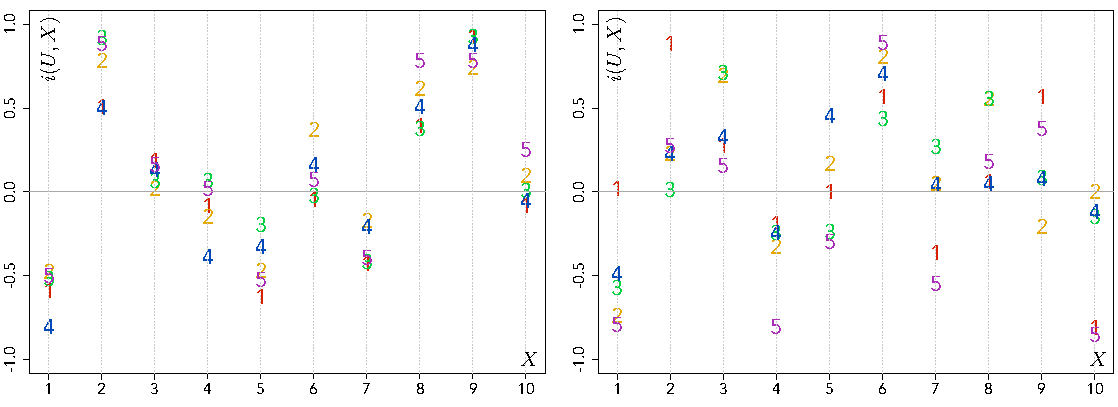
\epsfig{file=img/fig6_5, width=\textwidth}
\caption{Sample individual preferences of five participants whose profiles share an affinity of $\vartheta = 0.5$ (left) or $\vartheta = 1$ (right).}
\label{fig:bump}
\end{figure}

Figure~\ref{fig:bump} (left) represents the situation where $\vartheta = 0.5$; in this case all the individual preferences $i(U,X)$ for the first song are restricted to negative values in $[-0.9,-0.4]$, all the preferences for the second song are positive with values in $[0.4,0.9]$, all the preferences for the third song are medium with values in $[-0.2,0.3]$, and so on.
Figure~\ref{fig:bump} (right) illustrates the situation with a larger diameter $\vartheta = 1$; in this case the affinity is less evident. Note that when $\vartheta = 2$, the situation is identical to Fig.~\ref{fig:random} (right).

The evaluation of the experiment is run as in Sect.~\ref{sec:evaluation_of_this_technique}, with five participants listening to $25$ songs played on a channel, repeating the process $20$ times with different initial songs, and observing the values of $h(U,T)$ and $q(U,T)$ at each iteration.

\subsection{Results} % (fold)
\label{sub:results44}

Figure~\ref{fig:bump2} (left) shows the results when $\vartheta = 0.5$, that is, when participants have a quite strong affinity in musical taste. 
Compared to Fig.~\ref{fig:default} (right) (audience with no musical homogeneity), the results improve with respect to both the average individual preference (increased to $\overline{h(U,T)} = 0.86$) and the variance among different users (the standard deviation decreases to $0.02$).
%
\begin{figure}[bthp]
\centering \setlength{\abovecaptionskip}{3pt}
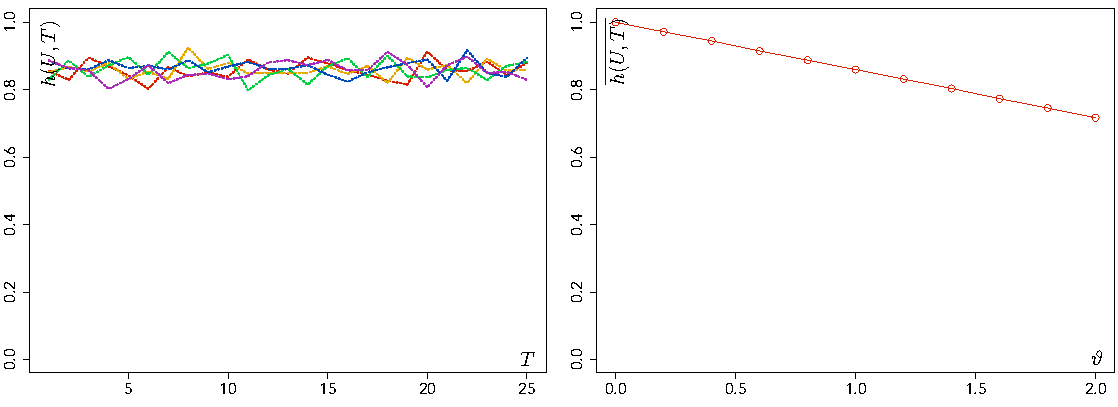
\epsfig{file=img/fig6_6, width=\textwidth}
\caption{Individual preferences for songs played when $\vartheta = 0.5$ (left) and correlation between affinity degree and average preferences (right).}
\label{fig:bump2}
\end{figure}

The relationship between group homogeneity and satisfaction is illustrated in Fig.~\ref{fig:bump2} (right), which shows how poolcasting is better able to deliver songs the audience strongly likes when the value of $\vartheta$ is small.
In the real world, a group of people listening to the same radio channel is expected to present some homogeneity in their musical taste, in which case the performance of poolcasting improves noticeably.

% subsection group_affinity (end)


\section{Scalability} % (fold)
\label{sub:scalability}

The next experiment evaluates the impact of the size of the audience over the group satisfaction.
The previous sections have only considered channels with five listeners; this section investigates whether adapting content for less or more people can affect the performance of poolcasting.

%Intuitively, adapting content for a few users should be simpler than adapting content for many users, especially when they have different preferences. This hypothesis is tested hereafter.

The evaluation is run using two new sets of artificial listeners: the first contains only two user profiles while the second simulates a group of twenty people. 
As in Sect.\ref{sec:evaluation_of_this_technique}, profiles are generated assigning random values in $[-1,1]$ to the individual preference $i(U,X)$ of each person for each song.
A channel is run for the duration of $25$ songs, the process repeated $20$ times and the satisfaction degrees $q(U,T)$ are analysed.

\subsection{Results} % (fold)
\label{sub:results345}

Figure~\ref{fig:size} shows the satisfaction degrees of the participants in a group of size 2 (left) and size 20 (right). 

Compared to the group of size 5 represented in Fig.~\ref{fig:default} (right), the satisfaction degrees are higher in Fig.~\ref{fig:size} (left) and lower in Fig.~\ref{fig:size} (right).
In other words, poolcasting has it easier to adapt content for smaller groups than for larger groups. This makes sense since the more the listeners, the more the music preferences to fulfil, and the harder to satisfy the entire audience.
Specifically, the average satisfaction degree decreases from
$\overline{q(U,T)} = 0.84$ with size 2, to $\overline{q(U,T)} = 0.72$ with size 5, to $\overline{q(U,T)} = 0.61$ with size 20.
%
\begin{figure}[bthp]
\centering \setlength{\abovecaptionskip}{3pt}
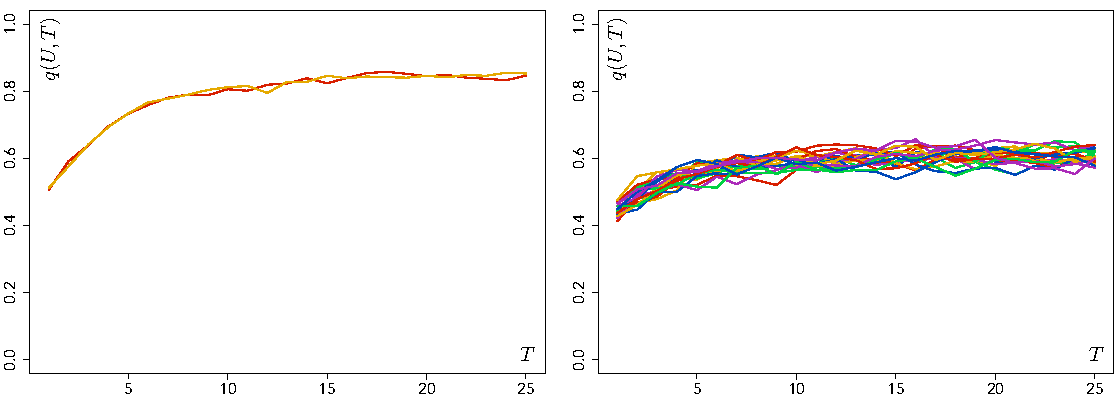
\epsfig{file=img/fig6_8, width=\textwidth}
\caption{Satisfaction degrees for a channel with 2 participants (left) or 20 listeners (right).}
\label{fig:size}
\end{figure}

More interesting, though, is that the variance between participants remains small even when the size of the group grows.
The lines plotted in Fig.~\ref{fig:size} (right) are all very close and stable over time, meaning that poolcasting is able to keep a good balance of the satisfactions of all the listeners in the long run.

Although one might conclude from this experiment that poolcasting can only be applied to radio channels with a small audience, this conclusion is not correct for a series of reasons.

Firstly, this section has focused only on a worst case scenario where all the listeners have random music preferences. 
In the real world, members of the same channel typically share some musical affinity, which makes it easier to find songs that satisfy multiple listeners at the same time.
As a consequence, group satisfaction is not always as badly affected by the group size as illustrated in Fig.~\ref{fig:size} (right).


Secondly, the experiment has been run on a channel with no filters, playing songs from every genre, tag or period. 
However most online radio stations restrict the music played to a specific set of songs (e.g. a `Rock' channel) to attract a public with a certain homogeneity in musical taste. 
As observed in Sect.~\ref{sub:concordance}, the stronger the affinity in the music profiles of the participants, the higher the satisfaction degree that poolcasting can provide, even for large groups.

%Thirdly, participants are free to join or leave a channel at different moments and, most importantly, to create new channels if they do not like the music played on existing ones (see Sect.~\ref{sec:innovative_features}). If a channel becomes too populated and a group-customised musical sequence cannot be supplied, part of the audience can move to a newly created channel (e.g., a second `Rock' channel) where poolcasting will be able to deliver songs better customised for their profiles.

Lastly, populated channels can benefit the listeners in terms of music discovery.
A listener $U$ connected to a channel with a large audience is more exposed to unknown music, played because of the preferences of other participants. 
Even though unknown songs will not match the music profiles of $U$, causing a decrease in the satisfaction degree $q(U,T)$, the chance of discovering new music is seen as a positive trade off by many listeners.

% All the participants can easily reach a satisfaction of 100\% by listening to music \emph{on their own}, selected by hand from their personal libraries, but in this way they would miss out the social component of the radio. A radio channel with a large audience, on the other hand, offers them a sequence of group-customised songs, of which some they already know and like, and others they get to discover.

The advantage of poolcasting is that, even when the audience is very large, fairness is achieved keeping the satisfaction of all the listeners balanced in the long run.

%[ TO DO: Worst case scenario shows poolcasting can maintain certain levels of performance even in a worst case scenario. More realistic scenarios will show better overall satisfaction, with more `affinity' among users. The experiments show that scalability is very correlated with group affinity, so as the channel audience grows there may be situations where affinity in audience groups will suggest to split channels.]

% subsection observations10 (end)

% subsection scalability (end)

\section{Other parameters} % (fold)
\label{sec:other_parameters}

The experiments in this section evaluate the impact of three other parameters of the poolcasting process over customisation and fairness. 

The first parameter is the retrieval size $\kappa$, which determines how many songs are selected in the retrieve process as `good candidates' to be played next. %, according to the properties of variety and smoothness.

The second parameter is the misery threshold $\mu$, which determines the minimum individual preference that any listener is willing to accept for any played song.

The third parameter is the initial satisfaction $\iota$, which determines the default value of $q(U,T)$ for a participant who has not yet listened to any song in the channel. 

All the experiments are performed under the conditions described in Sect.~\ref{sec:evaluation_of_this_technique}, with five artificial listeners with random music profiles.

%Another parameter that affects the outcome is the satisfaction decay $\chi$, which determines how rapidly each person forgets remote experiences. The effect of $\chi$ on the function $q(U,T)$ has already been examined in Sect.~\ref{sec:social-choice-problem}.
 

% section other_parameters (end)

\subsection{Retrieval size} % (fold)
\label{sub:retrieval_size}

The retrieval size $\kappa$, introduced in Sect.~\ref{sec:the_case_based_reasoning_selection_process}, indicates how many songs are selected in the retrieve step of the CBR process.
The larger the retrieval size $\kappa$, the more the candidate songs that are pre-selected to be played next, the higher the probability to find a candidate song the audience will like.
% This hypothesis that relates the value of $\kappa$ to the preference degrees $h(U,T)$ for the songs played is tested hereafter by running the evaluation process with different values of $\kappa$.

Figure~\ref{fig:default} (left) illustrated the outcome on individual preferences of running poolcasting with a default retrieval size of $\kappa = 15$. 
Figure~\ref{fig:retr_2} (left) evaluates the same process but with the parameter set to $\kappa = 30$. 
%
\begin{figure}[bthp]
\centering \setlength{\abovecaptionskip}{3pt}
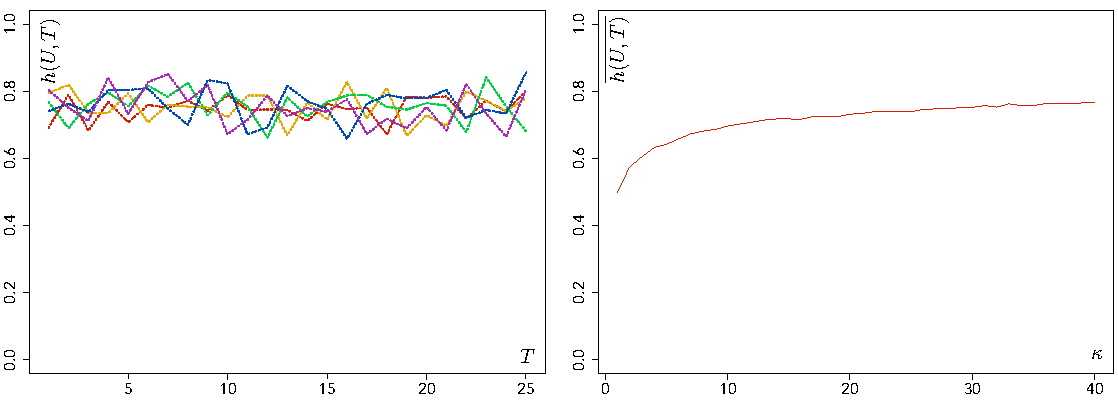
\epsfig{file=img/fig6_9, width=\textwidth}
\caption{Individual preferences for songs played when $\kappa = 30$ (left) and correlation between retrieval size and average preferences (right).}
\label{fig:retr_2}
\end{figure}

Having doubled the retrieval size, the average group preference increases but not noticeably, from $\overline{h(U,T)} = 0.72$ (with $\kappa = 15$) to 
$\overline{h(U,T)} = 0.76$ (with $\kappa = 30$).
%
Figure~\ref{fig:retr_2} (right) confirms this observation, showing the relationship between the retrieval size $\kappa$ and the average group preference $\overline{h(U,T)}$.
A clear improvement occurs in the lower range of intervals, but for values of $\kappa$ larger than 15 the average group preference remains quite stable.

For this reason, $\kappa = 15$ can be considered as a good retrieval size.
A smaller value would worsen the quality of the candidate set and, as a consequence, the quality of the played songs.
A larger value, on the other hand, would not improve much the quality and could decrease the performance of poolcasting, required to rank more candidate songs in real time.

Another good reason not to have a large retrieved set is that Poolcasting Web radio offers a Web page where listeners can send feedback for the candidate songs (see Fig.~\ref{fig:pwr_candidates}). 
If the list were too long, the audience would probably just ignore it, rather than stating a feedback which is very valuable to refine individual music profiles.

% subsection observations23 (end)

% subsection retrieval_size (end)

\subsection{Misery} % (fold)
\label{sub:misery}

Another parameter that affects the music selection process is the misery threshold $\mu \in [-1,1]$, introduced in Sect.~\ref{sub:how_we_fairly_aggregate_preferences}.
This value specifies the minimum preference degree that the audience is disposed to accept for a played song. 
For instance, if $\mu = 0$ then no song that any listener dislikes is allowed to play on the channel.
At the extreme, when $\mu = -1$ every song can be played; when $\mu = 1$ only songs that the whole public unconditionally loves can be played.

If the misery threshold is low, then every song can be played, even songs one participant detests (\emph{low minimum} individual preference) and everybody else loves (\emph{high group} preference). 
If the misery threshold is high, then only songs that no one detests (\emph{high minimum} individual preference) can be played, even if they have a \emph{low group} preference.

These two cases are illustrated in Fig.~\ref{fig:misery}, which represents the preference degrees of listeners for the songs played when the misery threshold is low ($\mu = -1$) or when the value is higher ($\mu = 0$).
The higher the threshold, the lower the average preference degree: $\overline{h(U,T)} = 0.73$ with $\mu = -1$ (left), $\overline{h(U,T)} = 0.59$ with $\mu = 0$ (right), while $\overline{h(U,T)} = 0.72$ with $\mu = -0.75$, as shown in Fig.~\ref{fig:default} (left).
%
\begin{figure}[bthp]
\centering \setlength{\abovecaptionskip}{3pt}
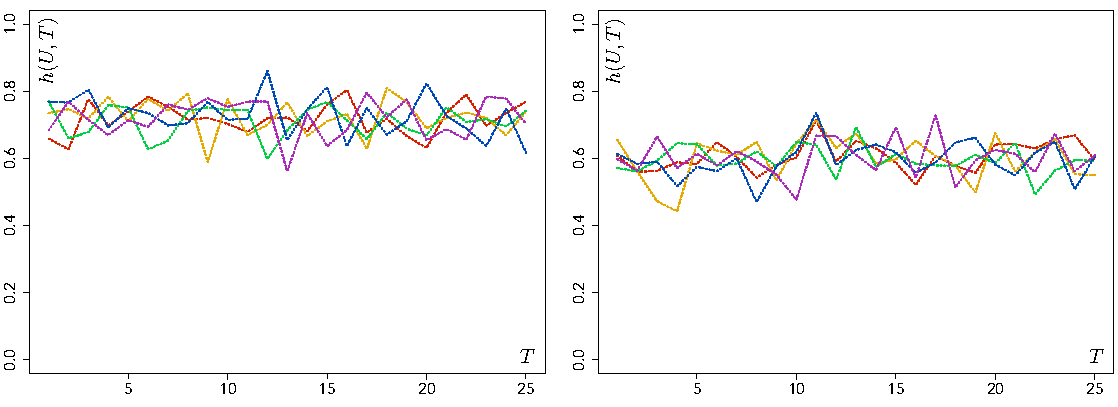
\epsfig{file=img/fig6_10, width=\textwidth}
\caption{Individual preferences for songs played when misery threshold $\mu = -1$ (left) or when $\mu = 0$ (right).}
\label{fig:misery}
\end{figure}

The lesson learnt is that the misery threshold is better kept small, since large values force poolcasting to select songs that will not bother anyone but that no one will really love either.

The threshold could as well be set to $\mu = -1$, to completely ignore the issue of misery. In fact, poolcasting listeners that do not like the songs played are already rewarded by the satisfaction-weighted aggregation.
By ignoring the issue of misery, poolcasting would make it impossible for malevolent participants to take control over the music played by strategically casting negative feedback for every song except those they would like to hear.

% subsection misery (end)


% subsection concordance (end)

% 
% 
% \subsection{Satisfaction decay} % (fold)
% \label{sub:satisfaction_decay}
% 
% Satisfaction is an emotion that decays over time, and the more recent experiences are those that affects us more. How much the remoteness of an election outcome influences the current satisfaction depends on the satisfaction decay. This graph shows how changing this factor modifies satisfaction over time; when this value equals 1, only the outcome of the last election decides the current satisfaction.
% 
% % subsection satisfaction_decay (end)
% 
% 
% 
% 
% \subsection{Weight to memory} % (fold)
% \label{sub:weight_to_memory}
% 
% This follows Experiment 4 to show how weighting the preferences of each person in relation to their preferences for previously selected items contribute to achieve fairness among different people. This graph shows how the standard deviation of satisfaction among the different persons is smaller keeping memory of past satisfactions (solid line), compared to the situations where each item is selected independently of the previous outcomes (dotted line).
% 
% Similarly to Experiment 4, individual preferences are generated with a random bimodal distribution; with three persons, two like some items and the third likes other ones; with five persons, three like some items, and the other two like other ones; and so on. The graph shows how the standard deviation of multiple satisfaction changes as the number of persons increase. Note that when the number is small (for example, 3 persons), the effect of memory is very clear, while it becomes less noticeable as the number of persons increase.
% 
% % subsection weight_to_memory (end)


\subsection{Initial satisfaction} % (fold)
\label{sub:initial_satisfaction}

The last parameter that can affect the outcome of poolcasting is the initial satisfaction $\iota \in [0,1]$, introduced in Sect.~\ref{sec:calculating_individual_satisfaction}.
This value defines the satisfaction degree of any person who has not yet listened to any song.

Figure~\ref{fig:iota} shows the effect of different values of $\iota$ on the satisfaction degrees of the participants: $\iota = 0$ (left) and $\iota = 1$ (right).
By comparison, Fig.~\ref{fig:default} (right) represented the default case where $\iota = 0.4$.
%
\begin{figure}[bthp]
\centering \setlength{\abovecaptionskip}{3pt}
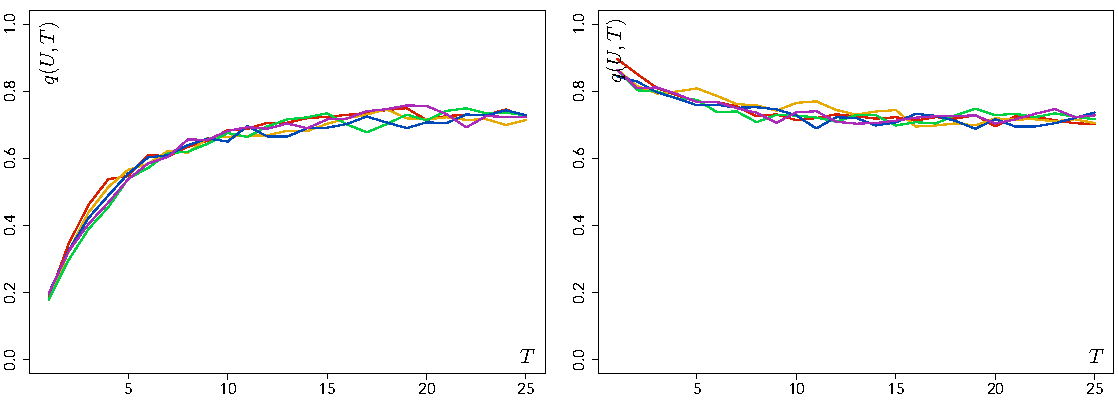
\epsfig{file=img/fig6_11, width=\textwidth}
\caption{Satisfaction degrees for songs played when participants have initial satisfaction $\iota = 0$ (left) or $\iota = 1$ (right).}
\label{fig:iota}
\end{figure}


The graph shows that the value of $\iota$ only affects individual satisfaction for the duration of the first songs.
After a while, the value is absorbed by the satisfaction decay and becomes irrelevant.
After $25$ songs, the satisfaction of the listeners is almost the same, independently of the value fixed for $\iota$.

The conclusion is that the value of $\iota$ does not affect satisfaction in the long run.
Using a default value of $\iota = 0.4$, slightly below the average, can help `boost' the importance of newcomer participants, so they can immediately listen to some songs they like when entering a channel.
This effect decays rapidly and, after a while, all the participants are treated equally independently of their initial satisfaction.

% subsection initial_satisfaction (end)

% section other_evaluations (end)





% section evaluation_of_this_technique (end)

% 
% 
% \section{The experiments with personalisation} % (fold)
% \label{sec:the_application3}
% 
% I had to create fake profiles. I matched the genres as the top tags of last.fm using \url{http://www.last.fm/group/Last.fm+Web+Services/forum/21604/_/285676}
% 
% % FAKE RATINGS FOR CLAUDIO:
% % insert into feedbacks(participant_id, candidate_id, song_id, artist_id, at_slot) select distinct 9, Null, song_id, artist_uid, Null from archives where song_id is not null and artist_uid is not null;
% % update feedbacks set degree = 2*rand()-1;
% 
% \subsection{Responsiveness} % (fold)
% \label{sub:responsiveness}
% 
% How fast the system adapts/changes?
% When user 1 enters, how long does it take to adapt? When he leaves and another one joins, what happens?
% 
% % subsection responsiveness (end)
% 
% 
% Now I repeat the same experiment, but I connect with a user to see if I influence and I get personalised sequences.
% 


% \subsection{Different influences} % (fold)
% \label{sub:different_influences}
% 
% Another evaluation is to have the channel with no filters at all and see where the music goes, in which styles, years, etc., whether it flows are stays still.
% In other words, I have a channel multi-genre and I enter with \emph{different} profiles, but ONE at the time, and see where music goes.
% 
% % subsection different_influences (end)
% 
% \subsection{Learning about personalisation over time} % (fold)
% \label{sub:learning_about_personalisation_over_time}
% 
% Explicit preferences also affect the customisation of the content for  a participant through time, at the beginning the system does not know a lot about a user, but as long as the same user continues to give ratings on the same channel, then the adaptation improves. 
% 
% another evaluation that I do with fake profiles is the following: I create these fake profiles and infer the preferences, and then I see how much satisfied the users are. now within the same channels I start giving explicit preferences, and our hypothesis is that the radio improves the customisation and the users are more satisfied. I do this and see that...
% 
% (this happens because the system has a larger knowledge)
% 
% this test I run with a channel made of a single user, has nothing to do with group customisation.
% 
% subsection learning_about_personalisation_over_time (end)

% section the_application3 (end)


% \section{Evaluation of fairness} % (fold)
% \label{sec:evaluation_of_desired_properties}
% 
% Here I should present the virtual work on the radio, with the desired properties and the parameters that affect them, and describe the problem of multi-genre channels.
% 
% \subsection{Scalability} % (fold)
% \label{sub:scalability}
% 
% How is this affected by the number of users? Number of songs?
% e.g. \emph{irony test}: I start with N songs and observe what happens when I increase/decrease the number of songs, or of users, or preferences.
% 
% If we split a large group in two, do they both increase satisfaction?
% 
% % subsection scalability (end)
% 
% \subsection{Average without misery} % (fold)
% \label{sub:average_without_misery}
% 
% Try to run the same channel but with a different aggregation method (e.g. plurality voting) and observe what happens to satisfactions.
% 
% % subsection average_without_misery (end)
% 
% \subsection{Own/other songs} % (fold)
% \label{sub:own_other_songs}
% 
% Show how often you get to listen to your own songs (fake profiles) and if this is equally distributed
% 
% % subsection own_other_songs (end)
% 
% \subsection{Individual vs. group} % (fold)
% \label{sub:individual_vs_group}
% 
% Under certain conditions, can the individual satisfaction be \emph{higher} in a group-addressed than in a personal system?
% 
% % subsection individual_vs_group (end)
% 
% 
% (explain the combination)
% 
% I do this test on the radio to see how many times the songs that is selected is selected because of song-to-song, song-.to-artustsm, a-to-a or random. once I have done this test I evaluate fairness like this., I create fake profiles with different preferences, each shanring a library, and on specific channels with different types of channel.
% \textbf{the first is channel defined with a genre}, like rock, an rpople likeing different shades of rock, and I see what happens and \textbf{how their satisfaction fluctuates} and if it's true that satisfaction enver falls below a certain threshold and what happens at this minimum satisfaction that I ever reach as I change some parameters, one of the parameter is the number of listeners. this is important because it's not the same ot satisfat a gorup of 2 or 10 persons, I try to see if 10 persons with different preferences can be satisfies, which is the maximum bnumber of people that can be satisfied, without changing the context which is defined by genre.
% 
% another test that I do is: what happens if the channel is not defined by a genre but by the period or by multiple genres or tags. if the context of the definition is very strict, then if you create a channel that is italian jazz music from the 50s and people go there, there you have strong restrictions, so if someone joins, more ore less he will be satisfied by every song played there, the selection is not very wide, while if you create a channel that is very wide, like music from the 80s, there you can have pop or rock or classical or soul, so you may start listening to pop, then people who like heavy metal join the channel, teh music should be more heavy metal,  if they leave and saoul lovers enter it hsould be more soul.
% the experiments here are to see if the music is adapted for the users. I have a channel defined as music from the 80s, withouth limitiation in terms of genres or tags, and in the bedinnging in this channel I have users who like sould and r\&b and our hypotheis is that the music that is selected from a repository that has any kind of genre available, contains more sould or r\&b music that the average. then they leave, and epople who love heavy metal enter the channel, and I want to see the number of sould and r\&b songs decrease, and metal increase. this is our hypothesis.
% and no one is very unsatisfied.
% 
% and I increase the number of users up to a limit.
% (and also I want to observe if smoothness is maintained in this transition)
% 
% 
% 
% 
% % section evaluation_of_desired_properties (end)
% 
% \section{Evaluation without a precise context} % (fold)
% \label{sec:evaluation_without_a_precise_context}
% 
% imagine now that I have in the previous situsation present at the same time, you have in a group people who like different genres, the channel as music form the 90s and 5 persons like sould r\&b and hip hop and 5 persons like rock or electronic rock or indie rock., in this situation you want to make everyone hwppy but also smoothness, I run experiement and see the sequence generated, and I don't just consider if smoothness is achieved or satisfaction is above a certain threshold, but I also look for a higher concept of smoothness, uintil now I have considered it just as song after this song, byut in this kind of sitatuion you also wanto smooth transition from a genre to the other. I ran the test and observe ...
% 
% (result)
% 
% it does not really occur wel the problem that I have is that if I just had one set, given smoothness as I have defined it then the songs tend to stay in the same area, if you are playing rock it tends to stay rock it does not navigate the whole network of artists, it tends to stay in one group becasuse there is no step to step transition from one song to the other, whay I would like to see is smyt in a more abstract senst that you go from a style to another and then go back and have smooth paths from one genre to the other. the point is that each artist is only. 
% 
% I want to see if this is true or not but I cannot because for each artists I have just one genre label, so I five songs labelled as rap and then five as rock and I don't know if in the middle there was a smooth transition from very very rap song to crossover song, and so on, this is what I would like, like a dj, if this is somethings in the middle it's good, not to jump from pure rock to pure rap. I would like to see this kind of bejhaviour in the radio. how can I do this? this is 
% 
% 
% % section evaluation_without_a_precise_context (end)
% 
% 
% % This is very unneeded! :-)
% % Evaluation may occur in labs or `in the wild'. Is there any difference? \cite{Baumann04} shows that ``there is no great difference between the two settings, and so no pressing need to implement an ecological approach to multimodal subjective similarity perception''.
% 
% 
% % subsection evaluation_of_desired_properties (end)
% 

%% This SECTION should be in the thesis, but the random profiles makes it
%% too difficult to estimate
% 
% \section{Discovery [TO DO: calculate and complete]} % (fold)
% \label{sub:serendipity}
% 
% So far, poolcasting has been evaluated with participants that had a defined (although random) preference for each available song. 
% Most of the times, though, a real listener does not know \emph{all} the songs the radio can broadcast and therefore does not have a clear preference for all them. Most of the times, the individual preference will simply be undefined.
% 
% What happens when a song is played that a person has never listened?
% He can either like it or not. 
% Intuitively, if a person is in a group of mind-alike fellows, it is more probable that he will like that song.
% This section evaluates exactly this.
% 
% %
% \begin{figure}[bthp]
% \centering \setlength{\abovecaptionskip}{3pt}
% \epsfig{file=img/discovery, width=\textwidth}
% \caption{Hiding some preferences [TO DO: change].}
% \label{fig:discovery}
% \end{figure}
% 
% Consider a set of listeners with random preferences.
% Consider that at each turn, poolcasting selects the next song by aggregating all the individual preferences but one. 
% That is, there is in turn a participant who \emph{has} musical preferences but does not \emph{disclose} them, so the song is selected without his contribution. After the song is selected and played, we check what this preference was. In other words, we select a song without the contribution of a user and hope that the user will like that song. We check this by considering the preference that user has (but had not disclosed).
% Intuitively, we will find higher preferences for groups with higher affinity. Let's check this out.
% 
% ...
% 

% subsection serendipity (end)


\section{Summary} % (fold)
\label{sec:contributions8}

This chapter has presented a series of evaluations of the poolcasting technique, both with real users and artificially created scenarios.

Experiments with real users have shown that radio channels can achieve variety and smoothness but some precautions have to be taken to prevent frustrating situations, like having the same sequence of songs repeated over time, or forcing listeners to wait too long for some preferred songs.
Interviewed subjects judged positively the compromise offered by the social experience in which participants do not listen only to favourite songs, but also to songs they ignore and will probably like since other like-minded listeners like them.

A series of evaluation tests has revealed how poolcasting behaves under different sets of constraints.
An initial experiment was run on a set of participants with random, independent music profiles, to which poolcasting could correctly provide a customised and fair musical sequence.
%
Although unrealistic, this experiment has shown that performance can be maintained at certain levels even in a worst-case scenario.

In a different experiment, the group was split between two discordant groups, and poolcasting could as well ensure fairness, playing songs that all the listeners liked in the long run.
On the contrary, a simple average voting strategy would only satisfy the majority, leaving the minority disappointed by the music played.

In the scenario where members of the audience share musical affinity, poolcasting works even better, finding more songs the audience appreciates. 
The size of the audience also affects the group satisfaction, which decreases as the size decreases, although the same balance is kept among different participants even when the group is large.
Satisfaction is maintained high if members of the audience tend to like the same kind of music.

% Poolcasting also helps people discover new music they possibly like, especially when the group is composed of mind-alike listeners.
Additional parameters that can affect the outcome were also evaluated (retrieval size, misery threshold, initial satisfaction) to find the most appropriate values for a good balance between performance and results.

% section contributions8(end)



% section what_can_be_evaluated (end)

%##########
% 
% \section{The evaluation of user modelling} % (fold)
% \label{sec:the_evaluation_of_user_modelling}
% 
% [REMOVE THIS]
% 
% Our hypothesis is that by observing the usage behaviour in terms of iTunes library I can infer implicit preferences, so to evaluate this I need real users, this is subjective, and I do the following: I recommend based on these preferences and see how people rate these songs after they have been played. the hypothesis is the following: \textbf{if i infer an implicit preference for a user and a specific song, i play that song on the radio and the rating of the user for that song will be positive}. if the rating is negative then this meant that our strategy is wrong. 
% 
% I did this during the test with real users and found that 
% 
% (at the end of this say that the results are not so good, and after a survey I find out that people normally don't rate lot their music, so the approach may be good, but I should use an even more implicit approach, and also people already remove bad songs from their libraries)
% 
% Also evaluate that ratings and play counts in iTunes are good indicators for the implicit preference
% 
% % section the_evaluation_of_user_modelling (end)


